\documentclass[]{elsarticle} %review=doublespace preprint=single 5p=2 column
%%% Begin My package additions %%%%%%%%%%%%%%%%%%%
\usepackage[hyphens]{url}

  \journal{Journal of Memory and Language} % Sets Journal name


\usepackage{lineno} % add
\providecommand{\tightlist}{%
  \setlength{\itemsep}{0pt}\setlength{\parskip}{0pt}}

\usepackage{graphicx}
%%%%%%%%%%%%%%%% end my additions to header

\usepackage[T1]{fontenc}
\usepackage{lmodern}
\usepackage{amssymb,amsmath}
\usepackage{ifxetex,ifluatex}
\usepackage{fixltx2e} % provides \textsubscript
% use upquote if available, for straight quotes in verbatim environments
\IfFileExists{upquote.sty}{\usepackage{upquote}}{}
\ifnum 0\ifxetex 1\fi\ifluatex 1\fi=0 % if pdftex
  \usepackage[utf8]{inputenc}
\else % if luatex or xelatex
  \usepackage{fontspec}
  \ifxetex
    \usepackage{xltxtra,xunicode}
  \fi
  \defaultfontfeatures{Mapping=tex-text,Scale=MatchLowercase}
  \newcommand{\euro}{€}
\fi
% use microtype if available
\IfFileExists{microtype.sty}{\usepackage{microtype}}{}
\bibliographystyle{elsarticle-harv}
\usepackage{color}
\usepackage{fancyvrb}
\newcommand{\VerbBar}{|}
\newcommand{\VERB}{\Verb[commandchars=\\\{\}]}
\DefineVerbatimEnvironment{Highlighting}{Verbatim}{commandchars=\\\{\}}
% Add ',fontsize=\small' for more characters per line
\usepackage{framed}
\definecolor{shadecolor}{RGB}{248,248,248}
\newenvironment{Shaded}{\begin{snugshade}}{\end{snugshade}}
\newcommand{\AlertTok}[1]{\textcolor[rgb]{0.94,0.16,0.16}{#1}}
\newcommand{\AnnotationTok}[1]{\textcolor[rgb]{0.56,0.35,0.01}{\textbf{\textit{#1}}}}
\newcommand{\AttributeTok}[1]{\textcolor[rgb]{0.77,0.63,0.00}{#1}}
\newcommand{\BaseNTok}[1]{\textcolor[rgb]{0.00,0.00,0.81}{#1}}
\newcommand{\BuiltInTok}[1]{#1}
\newcommand{\CharTok}[1]{\textcolor[rgb]{0.31,0.60,0.02}{#1}}
\newcommand{\CommentTok}[1]{\textcolor[rgb]{0.56,0.35,0.01}{\textit{#1}}}
\newcommand{\CommentVarTok}[1]{\textcolor[rgb]{0.56,0.35,0.01}{\textbf{\textit{#1}}}}
\newcommand{\ConstantTok}[1]{\textcolor[rgb]{0.00,0.00,0.00}{#1}}
\newcommand{\ControlFlowTok}[1]{\textcolor[rgb]{0.13,0.29,0.53}{\textbf{#1}}}
\newcommand{\DataTypeTok}[1]{\textcolor[rgb]{0.13,0.29,0.53}{#1}}
\newcommand{\DecValTok}[1]{\textcolor[rgb]{0.00,0.00,0.81}{#1}}
\newcommand{\DocumentationTok}[1]{\textcolor[rgb]{0.56,0.35,0.01}{\textbf{\textit{#1}}}}
\newcommand{\ErrorTok}[1]{\textcolor[rgb]{0.64,0.00,0.00}{\textbf{#1}}}
\newcommand{\ExtensionTok}[1]{#1}
\newcommand{\FloatTok}[1]{\textcolor[rgb]{0.00,0.00,0.81}{#1}}
\newcommand{\FunctionTok}[1]{\textcolor[rgb]{0.00,0.00,0.00}{#1}}
\newcommand{\ImportTok}[1]{#1}
\newcommand{\InformationTok}[1]{\textcolor[rgb]{0.56,0.35,0.01}{\textbf{\textit{#1}}}}
\newcommand{\KeywordTok}[1]{\textcolor[rgb]{0.13,0.29,0.53}{\textbf{#1}}}
\newcommand{\NormalTok}[1]{#1}
\newcommand{\OperatorTok}[1]{\textcolor[rgb]{0.81,0.36,0.00}{\textbf{#1}}}
\newcommand{\OtherTok}[1]{\textcolor[rgb]{0.56,0.35,0.01}{#1}}
\newcommand{\PreprocessorTok}[1]{\textcolor[rgb]{0.56,0.35,0.01}{\textit{#1}}}
\newcommand{\RegionMarkerTok}[1]{#1}
\newcommand{\SpecialCharTok}[1]{\textcolor[rgb]{0.00,0.00,0.00}{#1}}
\newcommand{\SpecialStringTok}[1]{\textcolor[rgb]{0.31,0.60,0.02}{#1}}
\newcommand{\StringTok}[1]{\textcolor[rgb]{0.31,0.60,0.02}{#1}}
\newcommand{\VariableTok}[1]{\textcolor[rgb]{0.00,0.00,0.00}{#1}}
\newcommand{\VerbatimStringTok}[1]{\textcolor[rgb]{0.31,0.60,0.02}{#1}}
\newcommand{\WarningTok}[1]{\textcolor[rgb]{0.56,0.35,0.01}{\textbf{\textit{#1}}}}
\usepackage{graphicx}
\ifxetex
  \usepackage[setpagesize=false, % page size defined by xetex
              unicode=false, % unicode breaks when used with xetex
              xetex]{hyperref}
\else
  \usepackage[unicode=true]{hyperref}
\fi
\hypersetup{breaklinks=true,
            bookmarks=true,
            pdfauthor={},
            pdftitle={Assessing replication rates in journals of experimental linguistics},
            colorlinks=false,
            urlcolor=blue,
            linkcolor=magenta,
            pdfborder={0 0 0}}
\urlstyle{same}  % don't use monospace font for urls

\setcounter{secnumdepth}{0}
% Pandoc toggle for numbering sections (defaults to be off)
\setcounter{secnumdepth}{0}

% Pandoc citation processing
\newlength{\cslhangindent}
\setlength{\cslhangindent}{1.5em}
\newlength{\csllabelwidth}
\setlength{\csllabelwidth}{3em}
% for Pandoc 2.8 to 2.10.1
\newenvironment{cslreferences}%
  {}%
  {\par}
% For Pandoc 2.11+
\newenvironment{CSLReferences}[2] % #1 hanging-ident, #2 entry spacing
 {% don't indent paragraphs
  \setlength{\parindent}{0pt}
  % turn on hanging indent if param 1 is 1
  \ifodd #1 \everypar{\setlength{\hangindent}{\cslhangindent}}\ignorespaces\fi
  % set entry spacing
  \ifnum #2 > 0
  \setlength{\parskip}{#2\baselineskip}
  \fi
 }%
 {}
\usepackage{calc}
\newcommand{\CSLBlock}[1]{#1\hfill\break}
\newcommand{\CSLLeftMargin}[1]{\parbox[t]{\csllabelwidth}{#1}}
\newcommand{\CSLRightInline}[1]{\parbox[t]{\linewidth - \csllabelwidth}{#1}\break}
\newcommand{\CSLIndent}[1]{\hspace{\cslhangindent}#1}

% Pandoc header



\begin{document}
\begin{frontmatter}

  \title{Assessing replication rates in journals of experimental
linguistics}
    \author[University of Osnabrück]{Kristina Kobrock\corref{1}}
   \ead{kkobrock@uni-osnabrueck.de} 
    \author[University of Oslo]{Timo B. Roettger}
  
      \address[University of Osnabrück]{Department, Street, City, State,
Zip}
    \address[University of Oslo]{Department, Street, City, State, Zip}
      \cortext[1]{Corresponding Author}
  
  \begin{abstract}
  This is the abstract. \textasciitilde150 words, avoid references,
  optional graphical abstract, keywords (max. 6, avoid abbreviations, AE
  spelling)

  It consists of two paragraphs.
  \end{abstract}
  
 \end{frontmatter}

\hypertarget{introduction}{%
\section{Introduction}\label{introduction}}

The replication and reproducibility of results is key to good scientific
practice. Yet, various scientific disciplines are currently facing what
is popularly referred to as a ``reproducibility'' or ``replication
crisis'' characterized by a small amount of published replication
studies and an increasing number of failed replication attempts
(\textbf{fidler\_reproducibility\_2018?}). Researchers from fields such
as psychology (Makel et al., 2012), education science (Makel and
Plucker, 2014), and special education research (Makel et al., 2016) have
assessed the amount of direct replications in their respective fields
and report alarmingly low replication rates ranging from 0.13\% in the
education sciences to 1.07\% in psychology publications. Coordinated
efforts to replicate published findings have uncovered surprisingly low
rates of successful replications ranging from 47\% in psychology (Open
Science Collaboration, 2015) to 61\% in economics (Camerer et al., 2016)
and 62\% in the social sciences (Camerer et al., 2018). A number of
failed replication attempts reported in various subfields of linguistics
indicate that the field is not immune to these raising concerns (e.g.~in
language comprehension: Papesh, 2015; predictive processing: Nieuwland
et al., 2018; among others: Chen, 2007; Stack et al., 2018; Westbury,
2018).

Experimental linguistics shares research practices that have been shown
to decrease the replicability of findings. Thus, there are raising
concerns about a similarly low number of replication studies conducted
and published in this field (e.g. Marsden et al., 2018; Roettger and
Baer-Henney, 2019). One driving factor for this phenomenon is an
asymmetric incentive system that rewards novel confirmatory findings
more than direct replications and null results. This leads to an
abundance of positive findings in the absence of possible conflicting
negative evidence (see also e.g. \textbf{fanelli\_pressures\_2010?}). In
order to thoroughly understand and be able to address this problem, it
is important to assess the number of replication attempts and their
contributing factors.

In order to evaluate the replication rate in experimental linguistics,
the present study assessed the frequency and typology of replication
studies that have been published in a representative sample of
experimental linguistic journals from their beginnings until 2020. The
study consisted of two parts: First, the frequency of self-reported
replication attempts across 100 linguistic journals were assessed and
the rate of replication mention was related to factors like journal
impact factor, publishing policy and publication access. Second, the
type of replication studies (direct, partial, conceptual) published in a
subset of 20 journals was investigated and their frequency was related
to factors like the year of publication, and the citation and
publication year of the initial study.

\hypertarget{overview-analysis-rate-of-replication-mention}{%
\section{Overview analysis: rate of replication
mention}\label{overview-analysis-rate-of-replication-mention}}

The key dependent variable of the first part of this study was the rate
of replication mention for journals relevant to the field of
experimental linguistics. We intended to answer the following research
questions: How many replication studies have been published in journals
representative for experimental linguistic research? How did the rate
change over time and how does it relate to journal policy, impact
factor, and publication type?

\hypertarget{material-and-methods}{%
\subsubsection{Material and methods}\label{material-and-methods}}

The material and methods have been preregistered on Open Science
Framework and can be inspected \href{https://osf.io/9ceas/}{here:
https://osf.io/9ceas/}.

In order to determine the rates of replication mention for individual
journals, we drew on a method introduced by Makel et al. (2012). First,
a sample of 100 journals relevant to the field of experimental
linguistics has been identified by making use of the search engine
\href{https://webofknowledge.com}{``Web of Science''
(https://webofknowledge.com)}. We restricted the search results to
journals in the web of science category ``Linguistics'' which had at
least 100 articles published and a high ratio of articles containing the
term ``experiment*'' in title, abstract or keywords. All English
language articles from the full available range of complete years
(1945-2020) were taken into account. We selected the top 100 journals
according to their ratio of experimental studies. The full list of
journals can be inspected \href{https://osf.io/q2e9k/}{here:
https://osf.io/q2e9k/}. The procedure described above helped us to
identify journals relevant for the field of experimental linguistics.
But this procedure can only yield a rough approximation of relevant
articles published in the field and several articles might thus have
been overlooked and not been included in the analysis. As a second step,
the total number of articles containing the search term ``replicat*'' in
title, abstract or keywords was obtained via Web of Science search for
the 100 sampled journals. Following the method used by Makel et al.
(2012) the rates of replication mention are calculated by dividing the
number of articles containing the term ``replicat*'' by the total number
of articles for each journal. As we were only interested in experimental
linguistic studies, we only included articles containing the search term
``experiment*'' in this formula.

In order to relate the rate of replication mention to journal policies,
we further examined the journals' submission guidelines adopting a
procedure used by Martin and Clarke (2017). They grouped psychology
journals into four classes determined by what was stated in the
``instructions to authors'' and ``aims and scope'' sections on the
websites of the respective journals: (1) Journals which stated that they
accepted replications; (2) Journals which did not state they accepted
replications but did not discourage replications either; (3) Journals
which implicitly discouraged replications through the use of emphasis on
the scientific originality of submissions, (4) Journals which actively
discouraged replications by stating explicitly that they did not accept
replications for publication (Martin and Clarke, 2017, p. 3). For our
analysis, it was only relevant whether journals explicitly encouraged
replication studies or not. So we grouped (2)-(4) together.

Journal impact factors were extracted via Journal Citation Reports
(https://jcr.clarivate.com). The 2019 journal impact factors are
calculated by dividing the citations in 2019 to items published in 2017
and 2018 by the total number of citable items in 2017 and 2018.

Furthermore, we assessed via Web of Science whether journals published
open access. We distinguished between three categories: journals which
are listed in the Directory of Open Access Journals (DOAJ) (``DOAJ
gold''), journals with some articles being published as open access
articles (``partial'') and journals with no option to publish open
access (``no'').

\hypertarget{results}{%
\subsubsection{Results}\label{results}}

\begin{verbatim}
##                               Journals Ratio of experimental studies
## 1       JOURNAL OF MEMORY AND LANGUAGE                         60.34
## 2     LANGUAGE AND COGNITIVE PROCESSES                         50.96
## 3                       MENTAL LEXICON                         45.71
## 4                 LANGUAGE ACQUISITION                         39.61
## 5  LANGUAGE COGNITION AND NEUROSCIENCE                         38.81
## 6                 LABORATORY PHONOLOGY                         37.42
## 7    LANGUAGE LEARNING AND DEVELOPMENT                         36.17
## 8         NATURAL LANGUAGE ENGINEERING                         32.05
## 9    LECTURE NOTES IN COMPUTER SCIENCE                         30.67
## 10              LANGUAGE AND COGNITION                         29.17
##    Rate of replication mention
## 1                         9.39
## 2                         8.52
## 3                         2.08
## 4                         1.22
## 5                         6.99
## 6                         5.17
## 7                        11.76
## 8                         1.00
## 9                         0.00
## 10                        4.76
\end{verbatim}

\begin{verbatim}
##                                        Journals Rate of replication mention
## 1 HUMOR INTERNATIONAL JOURNAL OF HUMOR RESEARCH                       12.82
\end{verbatim}

\begin{Shaded}
\begin{Highlighting}[]
\FunctionTok{head}\NormalTok{(guidelines)}
\end{Highlighting}
\end{Shaded}

\begin{verbatim}
##                                                                               journals
## 1                                        HUMOR INTERNATIONAL JOURNAL OF HUMOR RESEARCH
## 2                                                    LANGUAGE LEARNING AND DEVELOPMENT
## 3                                                                           MORPHOLOGY
## 4 TRANSLATION & INTERPRETING THE INTERNATIONAL JOURNAL OF TRANSLATION AND INTERPRETING
## 5                                            JOURNAL OF LOGIC LANGUAGE AND INFORMATION
## 6                                                       JOURNAL OF MEMORY AND LANGUAGE
##   policy
## 1      3
## 2      3
## 3      3
## 4      3
## 5      2
## 6      3
##                                                                                    webpage
## 1                                            http://www.humorstudies.org/JournalCenter.htm
## 2 https://www.tandfonline.com/action/authorSubmission?show=instructions&journalCode=hlld20
## 3                                                   https://www.springer.com/journal/11525
## 4               http://trans-int.org/index.php/transint/about/submissions#authorGuidelines
## 5                                    https://www.springer.com/journal/10849/aims-and-scope
## 6                        https://www.journals.elsevier.com/journal-of-memory-and-language/
##   binary_policy             jif openaccess
## 1             0           0.711    partial
## 2             0           1.651    partial
## 3             0 not retrievable    partial
## 4             0 not retrievable  DOAJ gold
## 5             0           0.440    partial
## 6             0           3.893    partial
\end{verbatim}

\begin{Shaded}
\begin{Highlighting}[]
\NormalTok{no\_encourage }\OtherTok{\textless{}{-}}\NormalTok{ guidelines }\SpecialCharTok{\%\textgreater{}\%} 
  \FunctionTok{filter}\NormalTok{(binary\_policy }\SpecialCharTok{==} \DecValTok{1}\NormalTok{) }\SpecialCharTok{\%\textgreater{}\%} 
  \FunctionTok{count}\NormalTok{() }
\CommentTok{\# {-}{-}\textgreater{} only 2 out of 100 journals explicitly encourage submission of replication studies}
\end{Highlighting}
\end{Shaded}

\hypertarget{discussion}{%
\subsubsection{Discussion}\label{discussion}}

\begin{itemize}
\tightlist
\item
  too little replication attempts in experimental linguistics
\item
  journals guidelines generally don't encourage replication studies
\item
  \ldots{}
\end{itemize}

\hypertarget{detailed-analysis-types-and-contributing-factors}{%
\section{Detailed analysis: types and contributing
factors}\label{detailed-analysis-types-and-contributing-factors}}

The second part of the study aimed at obtaining a better understanding
of the underlying mechanisms of replication attempts published in the
field of experimental linguistics. Because the term ``replication'' is
commonly used in ambiguous ways, the articles that contained the search
term ``replicat*'' required further analysis to determine whether the
articles in question indeed reported a replication study or used the
term in a different way.

We were interested in which kinds of replication studies are published
and which factors contribute to their publication. We aimed at
investigating what types of replication studies are prevalent in the
field. We were further interested in the relationship of direct
replications and whether the paper was published as open access or not,
the number of citations of the initial study and the years between
publication of the initial study and the replication attempt.

\hypertarget{material-and-methods-1}{%
\subsubsection{Material and methods}\label{material-and-methods-1}}

The material and methods have been preregistered on Open Science
Framework and can be inspected \href{https://osf.io/9ceas/}{here:
https://osf.io/9ceas/}.

From the superset of 100 journals obtained above, the first 20 journals
(i.e.~those journals with the highest proportion of experimental
studies) were selected for a more detailed analysis while excluding
journals for which less than 2 hits (TS=(replicat*)) could be obtained
(see \href{https://osf.io/f3yp8/}{here} for a list of article counts per
journal: https://osf.io/f3yp8/). Because of the skewed distribution of
our sample (114 hits for Journal of Memory and Language, and less than
40 for all other journals), we randomly selected (see
\href{https://osf.io/6vfpe/}{here} for details) 50 out of the 114
articles for the Journal of Memory and Language to achieve a more
balanced distribution of papers across journals. The sampling procedure
above resulted in 210 possible self-labeled replication studies.

In a first step, we identified whether the article in question indeed
presented a replication study or not. The relevant parts of the papers
were title and abstract of the paper, sentences around occurrences of
the search term ``replicat'' as well as the paragraph before the Methods
section and the first paragraph of the Discussion section (following the
procedure specified by Makel et al. (2016)). If the authors explicitly
claimed that (one of) their research aim(s) was to replicate or
reproduce findings or methods of an initial study, this article was
treated as a replication. It then qualified for further analysis after
the coding scheme that can be viewed \href{https://osf.io/ct2xj/}{here}:
https://osf.io/ct2xj/.

When extracting number and types of changes made to the initial study,
we assumed that the authors of a replication study did not make any
drastic changes \emph{without} reporting them. The replication studies
were classified according to three types: direct replication (0
changes), partial replication (1 change) and conceptual replication (2
or more changes), following Marsden et al. (2018). We noted the nature
of the change as one of the following categories (yes/no): experimental
paradigm, sample, materials/experimental set-up, dependent variable,
independent variable, and control. We also noted the language under
investigation. The information on whether the article was published open
access as well as citation counts and years of publication for both
studies were obtained from Web of Science. An author overlap was
attested when one of the authors was a (co-)author on both articles.

\hypertarget{results-1}{%
\subsubsection{Results}\label{results-1}}

\begin{verbatim}
##   mean_years
## 1   8.810127
\end{verbatim}

\begin{verbatim}
##   median_years
## 1            7
\end{verbatim}

\begin{verbatim}
##   mean_cit_init
## 1      41.08108
\end{verbatim}

\begin{verbatim}
##   median_cit_init
## 1            19.5
\end{verbatim}

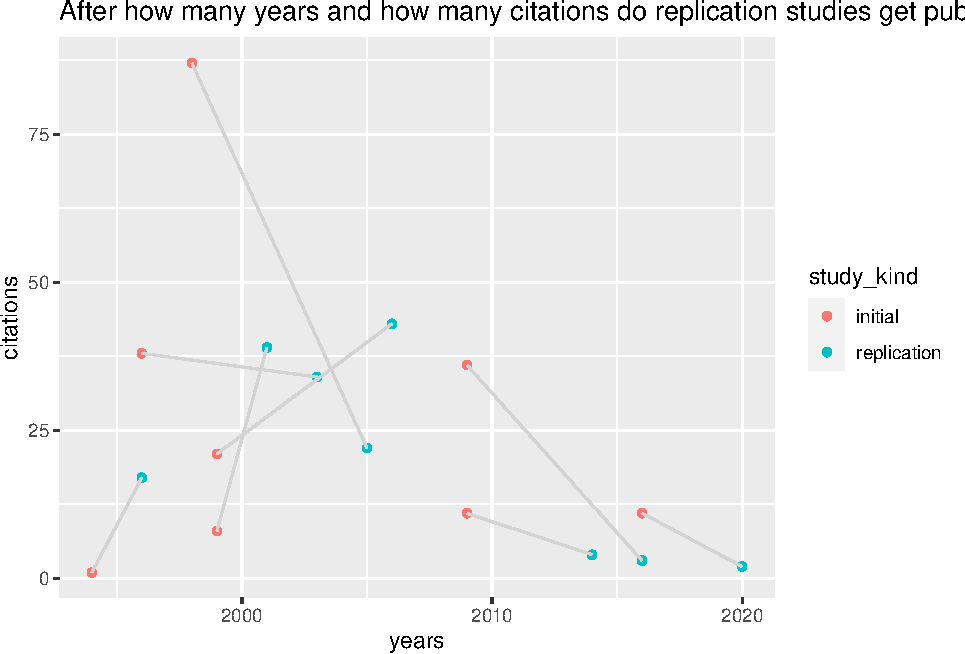
\includegraphics{ReplicationLing_files/figure-latex/plot cit and years direct-1.pdf}
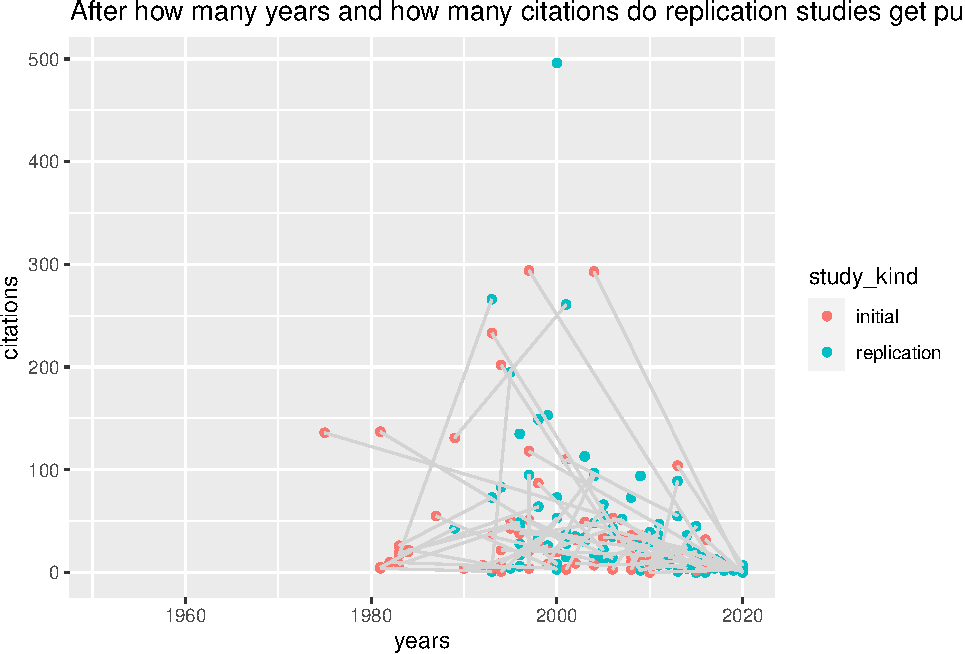
\includegraphics{ReplicationLing_files/figure-latex/plot cit and years all-1.pdf}

\begin{verbatim}
## type_replication
##            conceptual     direct    partial 
##       0.00       0.44       0.09       0.47
\end{verbatim}

\begin{verbatim}
##                 auth_overlap
## type_replication    0    1
##                  0.00 0.00
##       conceptual 0.18 0.26
##       direct     0.06 0.03
##       partial    0.24 0.24
\end{verbatim}

\begin{verbatim}
## [1] 0.04
\end{verbatim}

\hypertarget{discussion-1}{%
\subsubsection{Discussion}\label{discussion-1}}

\hypertarget{general-discussion}{%
\section{General discussion}\label{general-discussion}}

\begin{itemize}
\tightlist
\item
  compare rate of replication mention to previous studies in different
  fields --\textgreater{} broader picture
\end{itemize}

\hypertarget{appendices}{%
\section{Appendices}\label{appendices}}

identified as A, B, etc.

\hypertarget{references}{%
\section*{References}\label{references}}
\addcontentsline{toc}{section}{References}

\hypertarget{refs}{}
\begin{CSLReferences}{1}{0}
\leavevmode\vadjust pre{\hypertarget{ref-camerer_economics_2016}{}}%
Camerer, C.F., Dreber, A., Forsell, E., Ho, T.-H., Huber, J.,
Johannesson, M., Kirchler, M., Almenberg, J., Altmejd, A., Chan, T.,
Heikensten, E., Holzmeister, F., Imai, T., Isaksson, S., Nave, G.,
Pfeiffer, T., Razen, M., Wu, H., 2016. Evaluating replicability of
laboratory experiments in economics. Science 351, 1433--1436.
doi:\href{https://doi.org/10.1126/science.aaf0918}{10.1126/science.aaf0918}

\leavevmode\vadjust pre{\hypertarget{ref-camerer_socscience_2018}{}}%
Camerer, C.F., Dreber, A., Holzmeister, F., Ho, T.-H., Huber, J.,
Johanesson, M., Kirchler, M., Nave, G., Nosek, B.A., Pfeiffer, T.,
Altmejd, A., Buttrick, N., Chan, T., Chen, Y., Forsell, E., Gampa, A.,
Heikensten, E., Hummer, L., Imai, T., Isaksson, S., Manfredi, D., Rose,
J., Wagenmakers, E.-J., Wu, H., 2018. Evaluating the replicability of
social science experiments in nature and science between 2010 and 2015.
Nature 2, 637--644.
doi:\href{https://doi.org/10.1038/s41562-018-0399-z}{10.1038/s41562-018-0399-z}

\leavevmode\vadjust pre{\hypertarget{ref-chen_chinese_2007}{}}%
Chen, J.-Y., 2007. Do {Chinese} and {English} speakers think about time
differently? {Failure} of replicating {Boroditsky} (2001). Cognition
104, 427--436.

\leavevmode\vadjust pre{\hypertarget{ref-makel2014facts}{}}%
Makel, M.C., Plucker, J.A., 2014. Facts are more important than novelty:
Replication in the education sciences. Educational Researcher 43,
304--316.

\leavevmode\vadjust pre{\hypertarget{ref-makel_replications_2016}{}}%
Makel, M.C., Plucker, J.A., Freeman, J., Lombardi, A., Simonsen, B.,
Coyne, M., 2016. Replication of special education research: Necessary
but far too rare. Remedial and Special Education 37, 205--212.

\leavevmode\vadjust pre{\hypertarget{ref-makel_replications_2012}{}}%
Makel, M.C., Plucker, J.A., Hegarty, B., 2012. Replications in
psychology research: {How} often do they really occur? Perspectives on
Psychological Science 7, 537--542.

\leavevmode\vadjust pre{\hypertarget{ref-marsden_replication_2018}{}}%
Marsden, E., Morgan‐Short, K., Thompson, S., Abugaber, D., 2018.
Replication in {Second} {Language} {Research}: {Narrative} and
{Systematic} {Reviews} and {Recommendations} for the {Field}. Language
Learning 68, 321--391. doi:\href{https://doi.org/gc3h3b}{gc3h3b}

\leavevmode\vadjust pre{\hypertarget{ref-martinclarke_policies_2017}{}}%
Martin, G.N., Clarke, R.M., 2017. Are psychology journals
anti-replication? A snapshot of editorial practices. Frontiers in
Psychology 8.
doi:\href{https://doi.org/10.3389/fpsyg.2017.00523}{10.3389/fpsyg.2017.00523}

\leavevmode\vadjust pre{\hypertarget{ref-nieuwland_large-scale_2018}{}}%
Nieuwland, M.S., Politzer-Ahles, S., Heyselaar, E., Segaert, K., Darley,
E., Kazanina, N., Zu Wolfsthurn, S.V.G., Bartolozzi, F., Kogan, V., Ito,
A., Mézière, D., Barr, D.J., Rousselet, G.A., Ferguson, H.J.,
Bush-Moreno, S., Fu, X., Tuomainen, J., Kulakova, E., Husband, M.E.,
Donaldson, D.I., Kohút, Z., Rueschemeyer, S.-A., Huettig, F., 2018.
Large-scale replication study reveals a limit on probabilistic
prediction in language comprehension. eLife 7, e33468.
doi:\href{https://doi.org/10.7554/eLife.33468.001}{10.7554/eLife.33468.001}

\leavevmode\vadjust pre{\hypertarget{ref-open_science_collaboration_estimating_2015}{}}%
Open Science Collaboration, 2015. Estimating the reproducibility of
psychological science. Science 349.
doi:\href{https://doi.org/10.1126/science.aac4716}{10.1126/science.aac4716}

\leavevmode\vadjust pre{\hypertarget{ref-papesh_just_2015}{}}%
Papesh, M.H., 2015. Just out of reach: {On} the reliability of the
action-sentence compatibility effect. Journal of Experimental
Psychology: General 144, e116--e141.
doi:\href{https://doi.org/10.1037/xge0000125}{10.1037/xge0000125}

\leavevmode\vadjust pre{\hypertarget{ref-roettger2019toward}{}}%
Roettger, T.B., Baer-Henney, D., 2019. Toward a replication culture:
Speech production research in the classroom. Phonological Data and
Analysis 1, 1--23.

\leavevmode\vadjust pre{\hypertarget{ref-stack_failure_2018}{}}%
Stack, C.M.H., James, A.N., Watson, D.G., 2018. A failure to replicate
rapid syntactic adaptation in comprehension. Memory \& Cognition 46,
864--877.
doi:\href{https://doi.org/10.3758/s13421-018-0808-6}{10.3758/s13421-018-0808-6}

\leavevmode\vadjust pre{\hypertarget{ref-westbury_implicit_2018}{}}%
Westbury, C., 2018. Implicit sound symbolism effect in lexical access,
revisited: {A} requiem for the interference task paradigm. Journal of
Articles in Support of the Null Hypothesis 15, 1--12.

\end{CSLReferences}


\end{document}
